
\lecture{Prediction Intervals}{prediction-intervals}
\section{Prediction Intervals}

\title{Prediction Intervals}
\subtitle{What will it be?}

%\author{Kelly Black}
%\institute{Clarkson University}
\date{3 December 2014}

\begin{frame}
  \titlepage
\end{frame}

\begin{frame}
  \frametitle{Outline}
  \tableofcontents[hideothersubsections,sectionstyle=show/hide]
\end{frame}


\subsection{Clicker Quiz}


\iftoggle{clicker}{%
  \begin{frame}
    \frametitle{Clicker Quiz}

    \begin{columns}
      \column{.15\textwidth}

      \begin{tabular}{l|l}
        $X$ & $Y$ \\ \hline
        1 &  -4.7 \\
        2 & -15.4  \\
        3 &  -9.6 \\
        4 & -21.5 
      \end{tabular}

      \column{.44\textwidth}

      \begin{eqnarray*}
        \bar{x} & = & 2.5 \\
        \bar{y} & = & -12.8.
      \end{eqnarray*}

      \column{.44\textwidth}

      \only<1>{%
        \begin{eqnarray*}
          s_{xx} & = & ?, \\
          s_{yy} & = & 158.3, \\
          s_{xy} & = & -22.3.
        \end{eqnarray*}
      }
      \only<2>{%
        \begin{eqnarray*}
          s_{xx} & = & 5, \\
          s_{yy} & = & 158.3, \\
          s_{xy} & = & -22.3.
        \end{eqnarray*}
      }


    \end{columns}


    \vfill

    What is the value of $s_{xx}$? \\
    \begin{tabular}{l@{\hspace{3em}}l@{\hspace{3em}}l}
      A: 0 & B: 2.75 & C: 5
    \end{tabular}

    \vfill
    \vfill
    \vfill

  \end{frame}

}

\subsection{Inference On Predicted Value}


\begin{frame}
  \frametitle{Recall: Linear Regression}


  \begin{tabular}{r|r<{\onslide<2->}|r<{\onslide<3->}|r<{\onslide}} % 
    $X$ & $Y$ & $\hat{Y}$ & Residual \\ \hline
    $x_1$ & $y_1$ & $\hat{y}_1=\hat{\beta_1}x_1+\hat{\beta_0}$ & $\epsilon_1 = y_1-\hat{y}_1$ \\
    $x_2$ & $y_2$ & $\hat{y}_2=\hat{\beta_1}x_2+\hat{\beta_0}$ & $\epsilon_2 = y_2-\hat{y}_2$  \\
    $\vdots$ & $\vdots$ & $\vdots$ & $\vdots$  \\
    $x_n$ & $y_n$ & $\hat{y}_n=\hat{\beta_1}x_n+\hat{\beta_0}$ & $\epsilon_n = y_n-\hat{y}_n$
  \end{tabular}

  Calculate the following:
  \begin{eqnarray*}
    S_{xx} & = & \lp x_1 - \bar{x}\rp^2 + \cdots + \lp x_n - \bar{x} \rp^2, \\
    S_{yy} & = & \lp y_1 - \bar{y}\rp^2 + \cdots + \lp y_n - \bar{y} \rp^2, \\
    S_{xy} & = & \lp x_1 - \bar{x}\rp\lp y_1 - \bar{y}\rp + \cdots + \lp x_n - \bar{x} \rp\lp y_n - \bar{y}\rp, \\
    \hat{\beta_1} & = & \frac{S_{xy}}{S_{xx}}, \\
    \hat{\beta_0} & = & \bar{y} - \hat{\beta_1} \bar{x}, \\
    \only<4->
    {
      \hat{\sigma}^2_y & = & \frac{\lp y_1 - \hat{y}_1\rp^2 + \lp y_2 - \hat{y}_2\rp^2 + \cdots + \lp y_n - \hat{y}_n\rp^2 }{n-2}.
    }
  \end{eqnarray*}

\end{frame}


\begin{frame}
  \frametitle{Linear Regression}

    \begin{columns}
      \column{.15\textwidth}

      \begin{tabular}{l|l}
        $X$    & $Y$ \\ \hline
        $x_1$  & $y_1$  \\
        $x_2$  & $y_2$  \\
        \vdots & \vdots  \\
        $x_n$  & $y_n$
      \end{tabular}

      \column{.44\textwidth}

      \begin{eqnarray*}
        \bar{x} \\
        \bar{y} \\
        S_{xx} \\
        S_{yy} \\
        S_{xy} 
        \end{eqnarray*}

      \column{.44\textwidth}
      
      \begin{eqnarray*}
        y & = & \beta_1 x + \beta_0 + {\color{red}\epsilon} \\
        {\color{blue}\hat{\beta}_1} & = & \frac{S_{xy}}{S_{xx}} \\
        {\color{blue}\hat{\beta}_0} & = & \bar{y} - {\color{blue}\hat{\beta}_1} \bar{x} \\
        t & = & \frac{\hat{\beta}_1-\beta_1}{\lp\frac{\hat{\sigma}_y}{\sqrt{s_{xx}}}\rp},~df=n-2
      \end{eqnarray*}

    \end{columns}


      \only<2>{%

        Question: After calculating $\hat{\beta}_1$ and
        $\hat{\beta}_0$ we want to estimate the value of $y$ for a
        given value of $x$. What is the value of $y$?

        Problem: It depends on three random variables, $\hat{\beta}_1$,
        $\hat{\beta}_0$, and $\epsilon$.

      }



\end{frame}

\begin{frame}{The Predicted Value}

  \begin{definition}
    The \textit{predicted value} for $y$ at $x$ is
    \begin{eqnarray*}
      \hat{y} & = & \hat{\beta}_1 x + \hat{\beta}_0.
    \end{eqnarray*}
  \end{definition}

    \only<2>{%
      \centerline{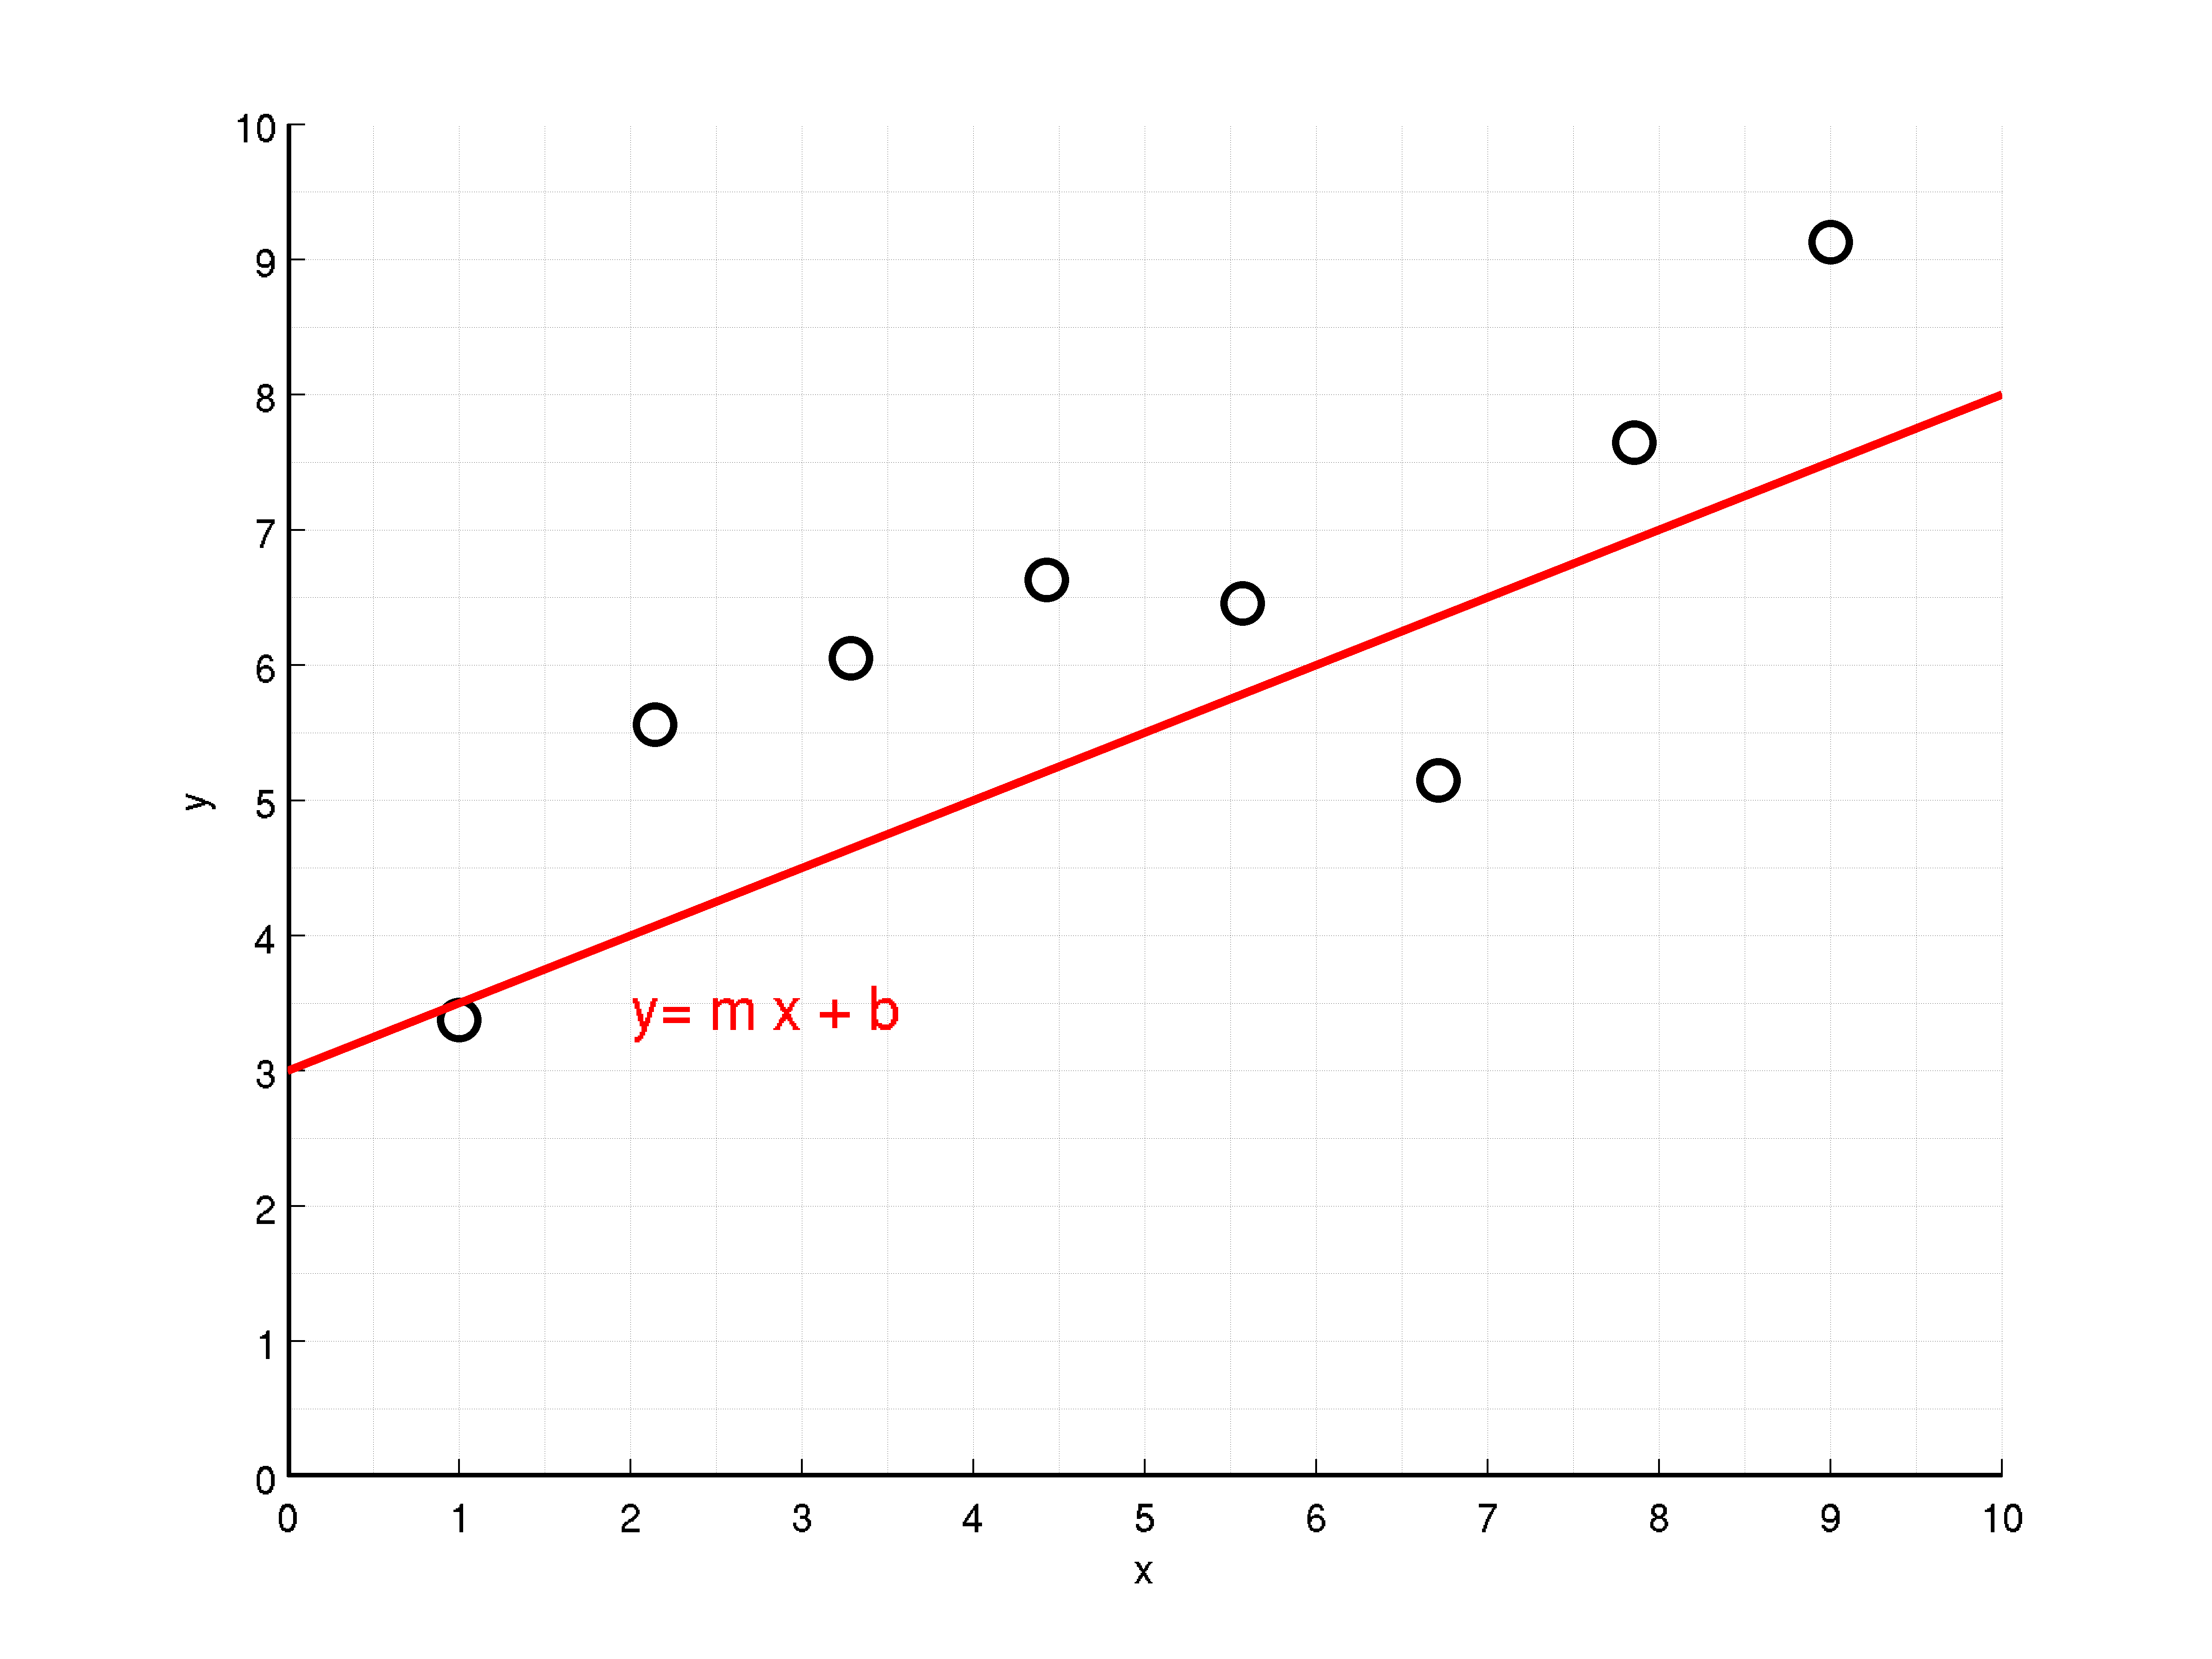
\includegraphics[width=5cm]{img/regressionInferenceOne}}
    }

    \only<3>{%
      \centerline{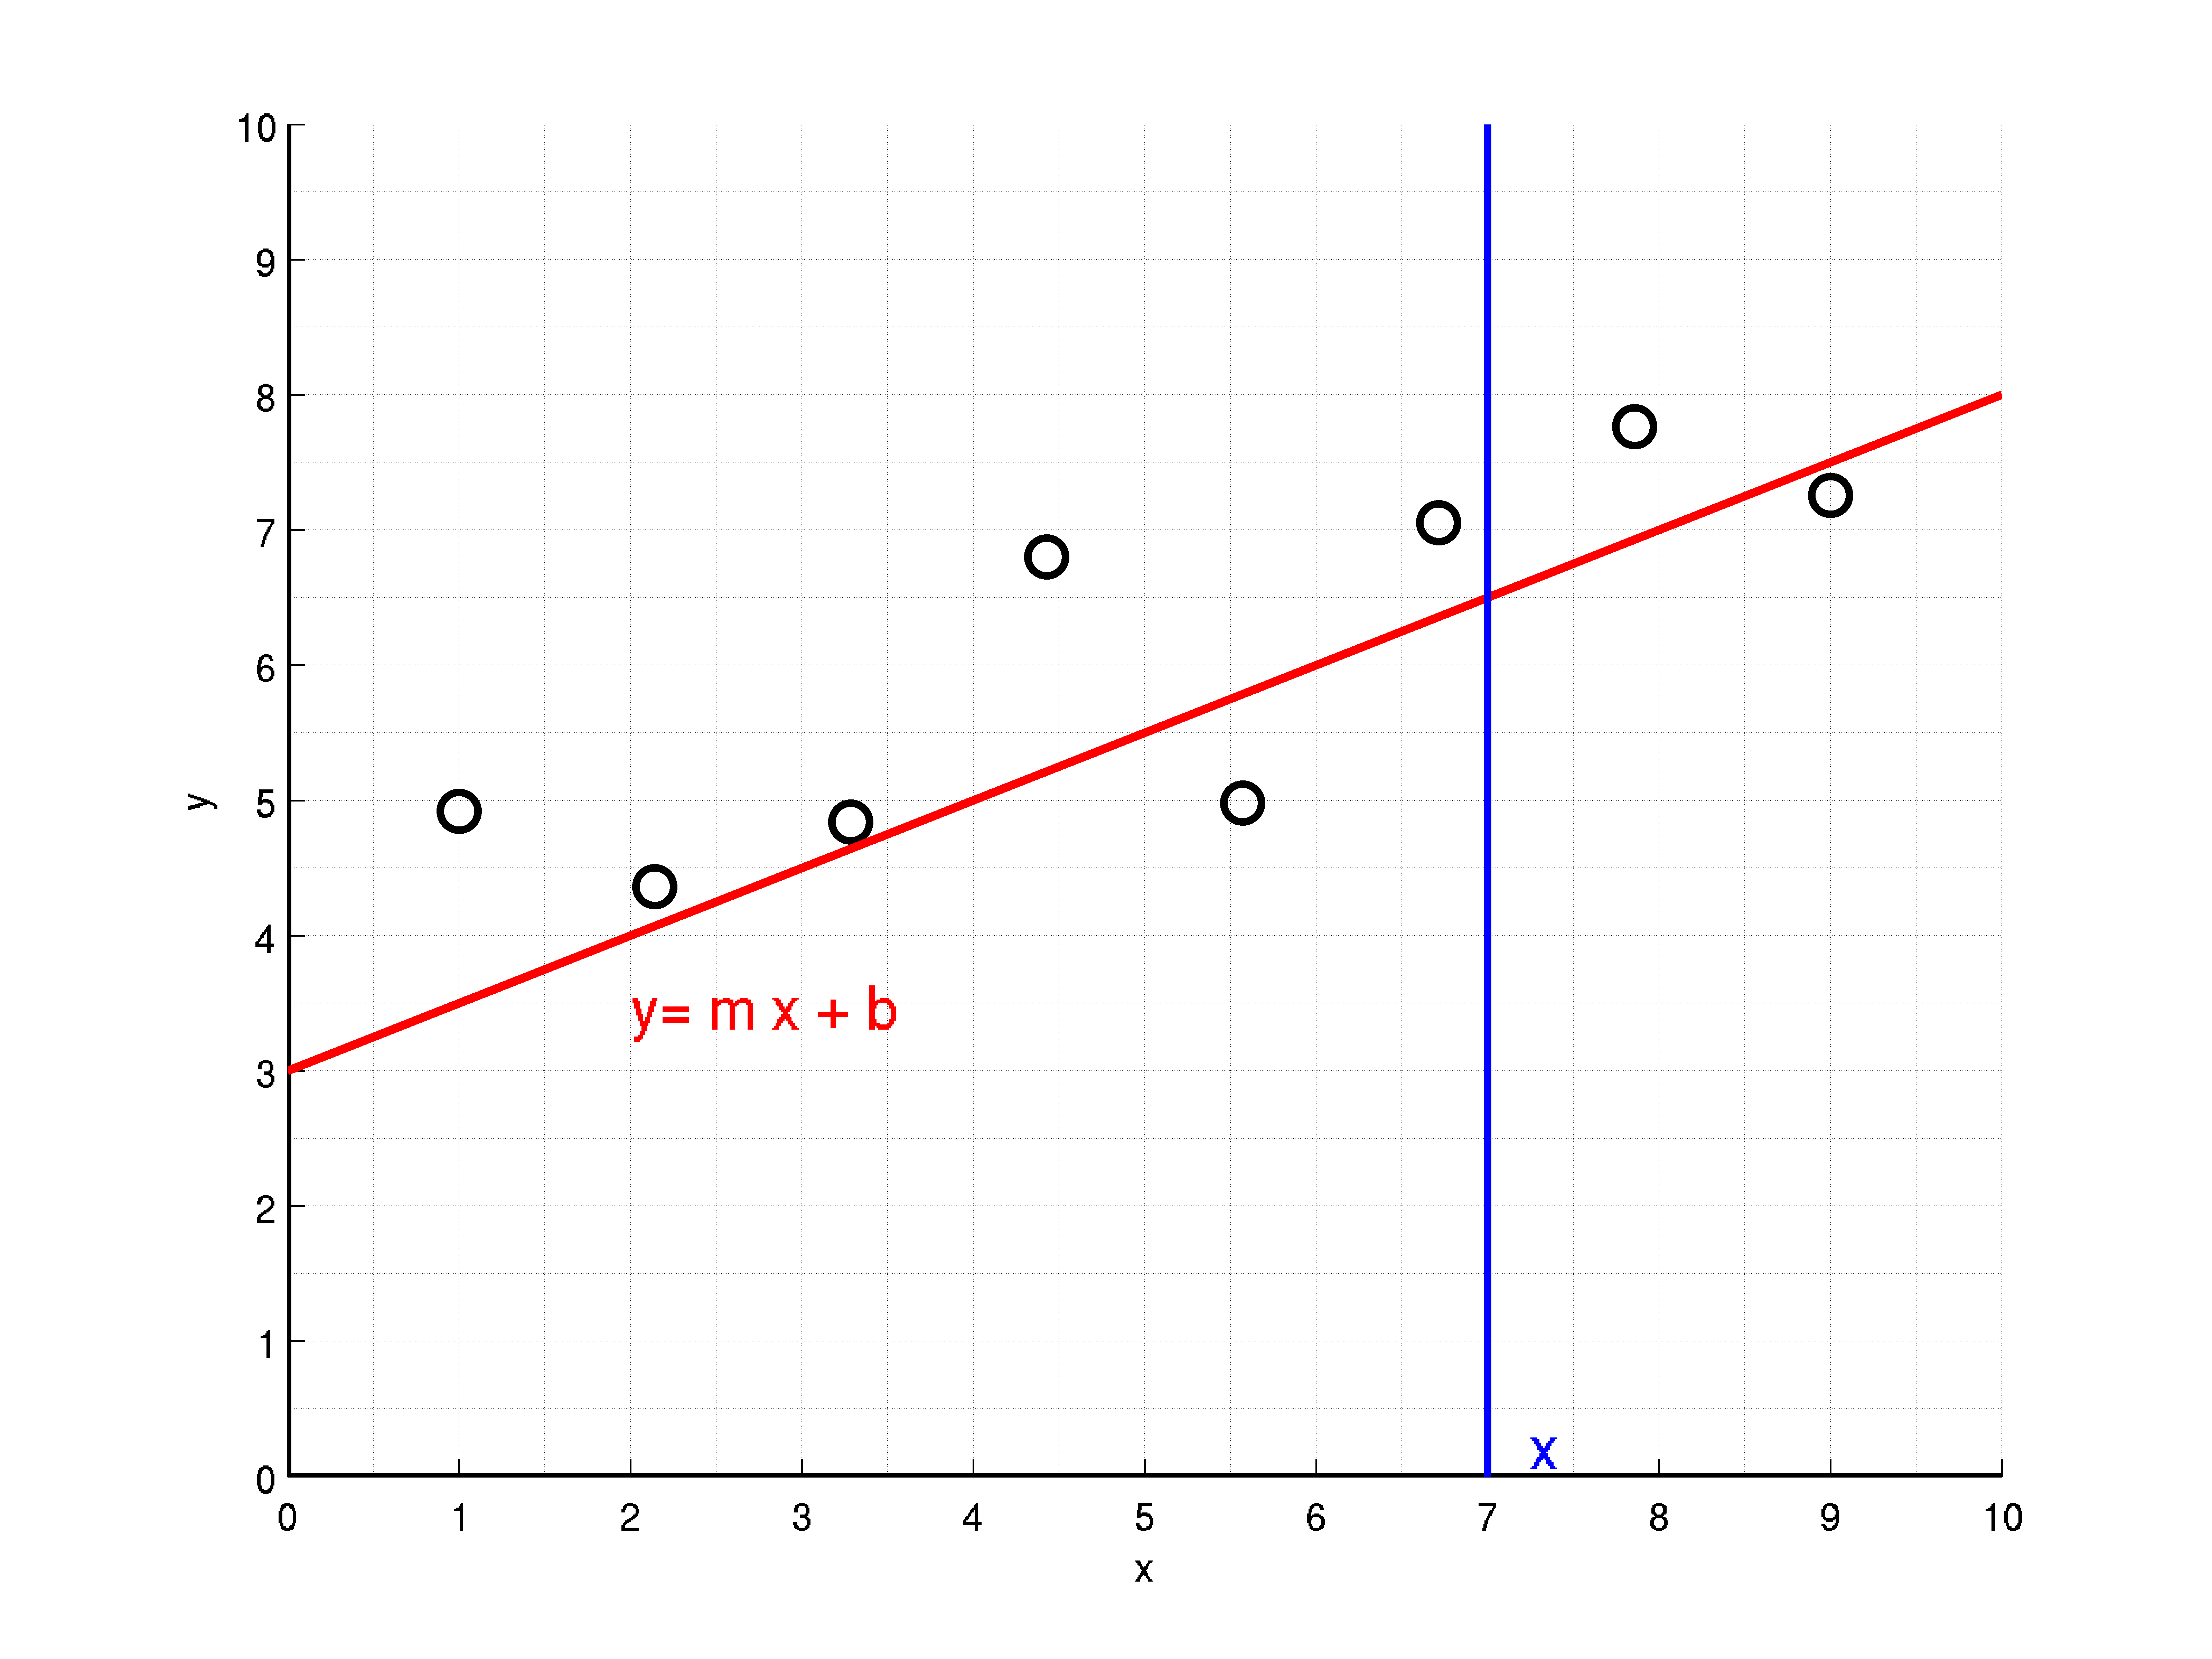
\includegraphics[width=5cm]{img/regressionInferenceTwo}}
    }

    \only<4>{%
      \centerline{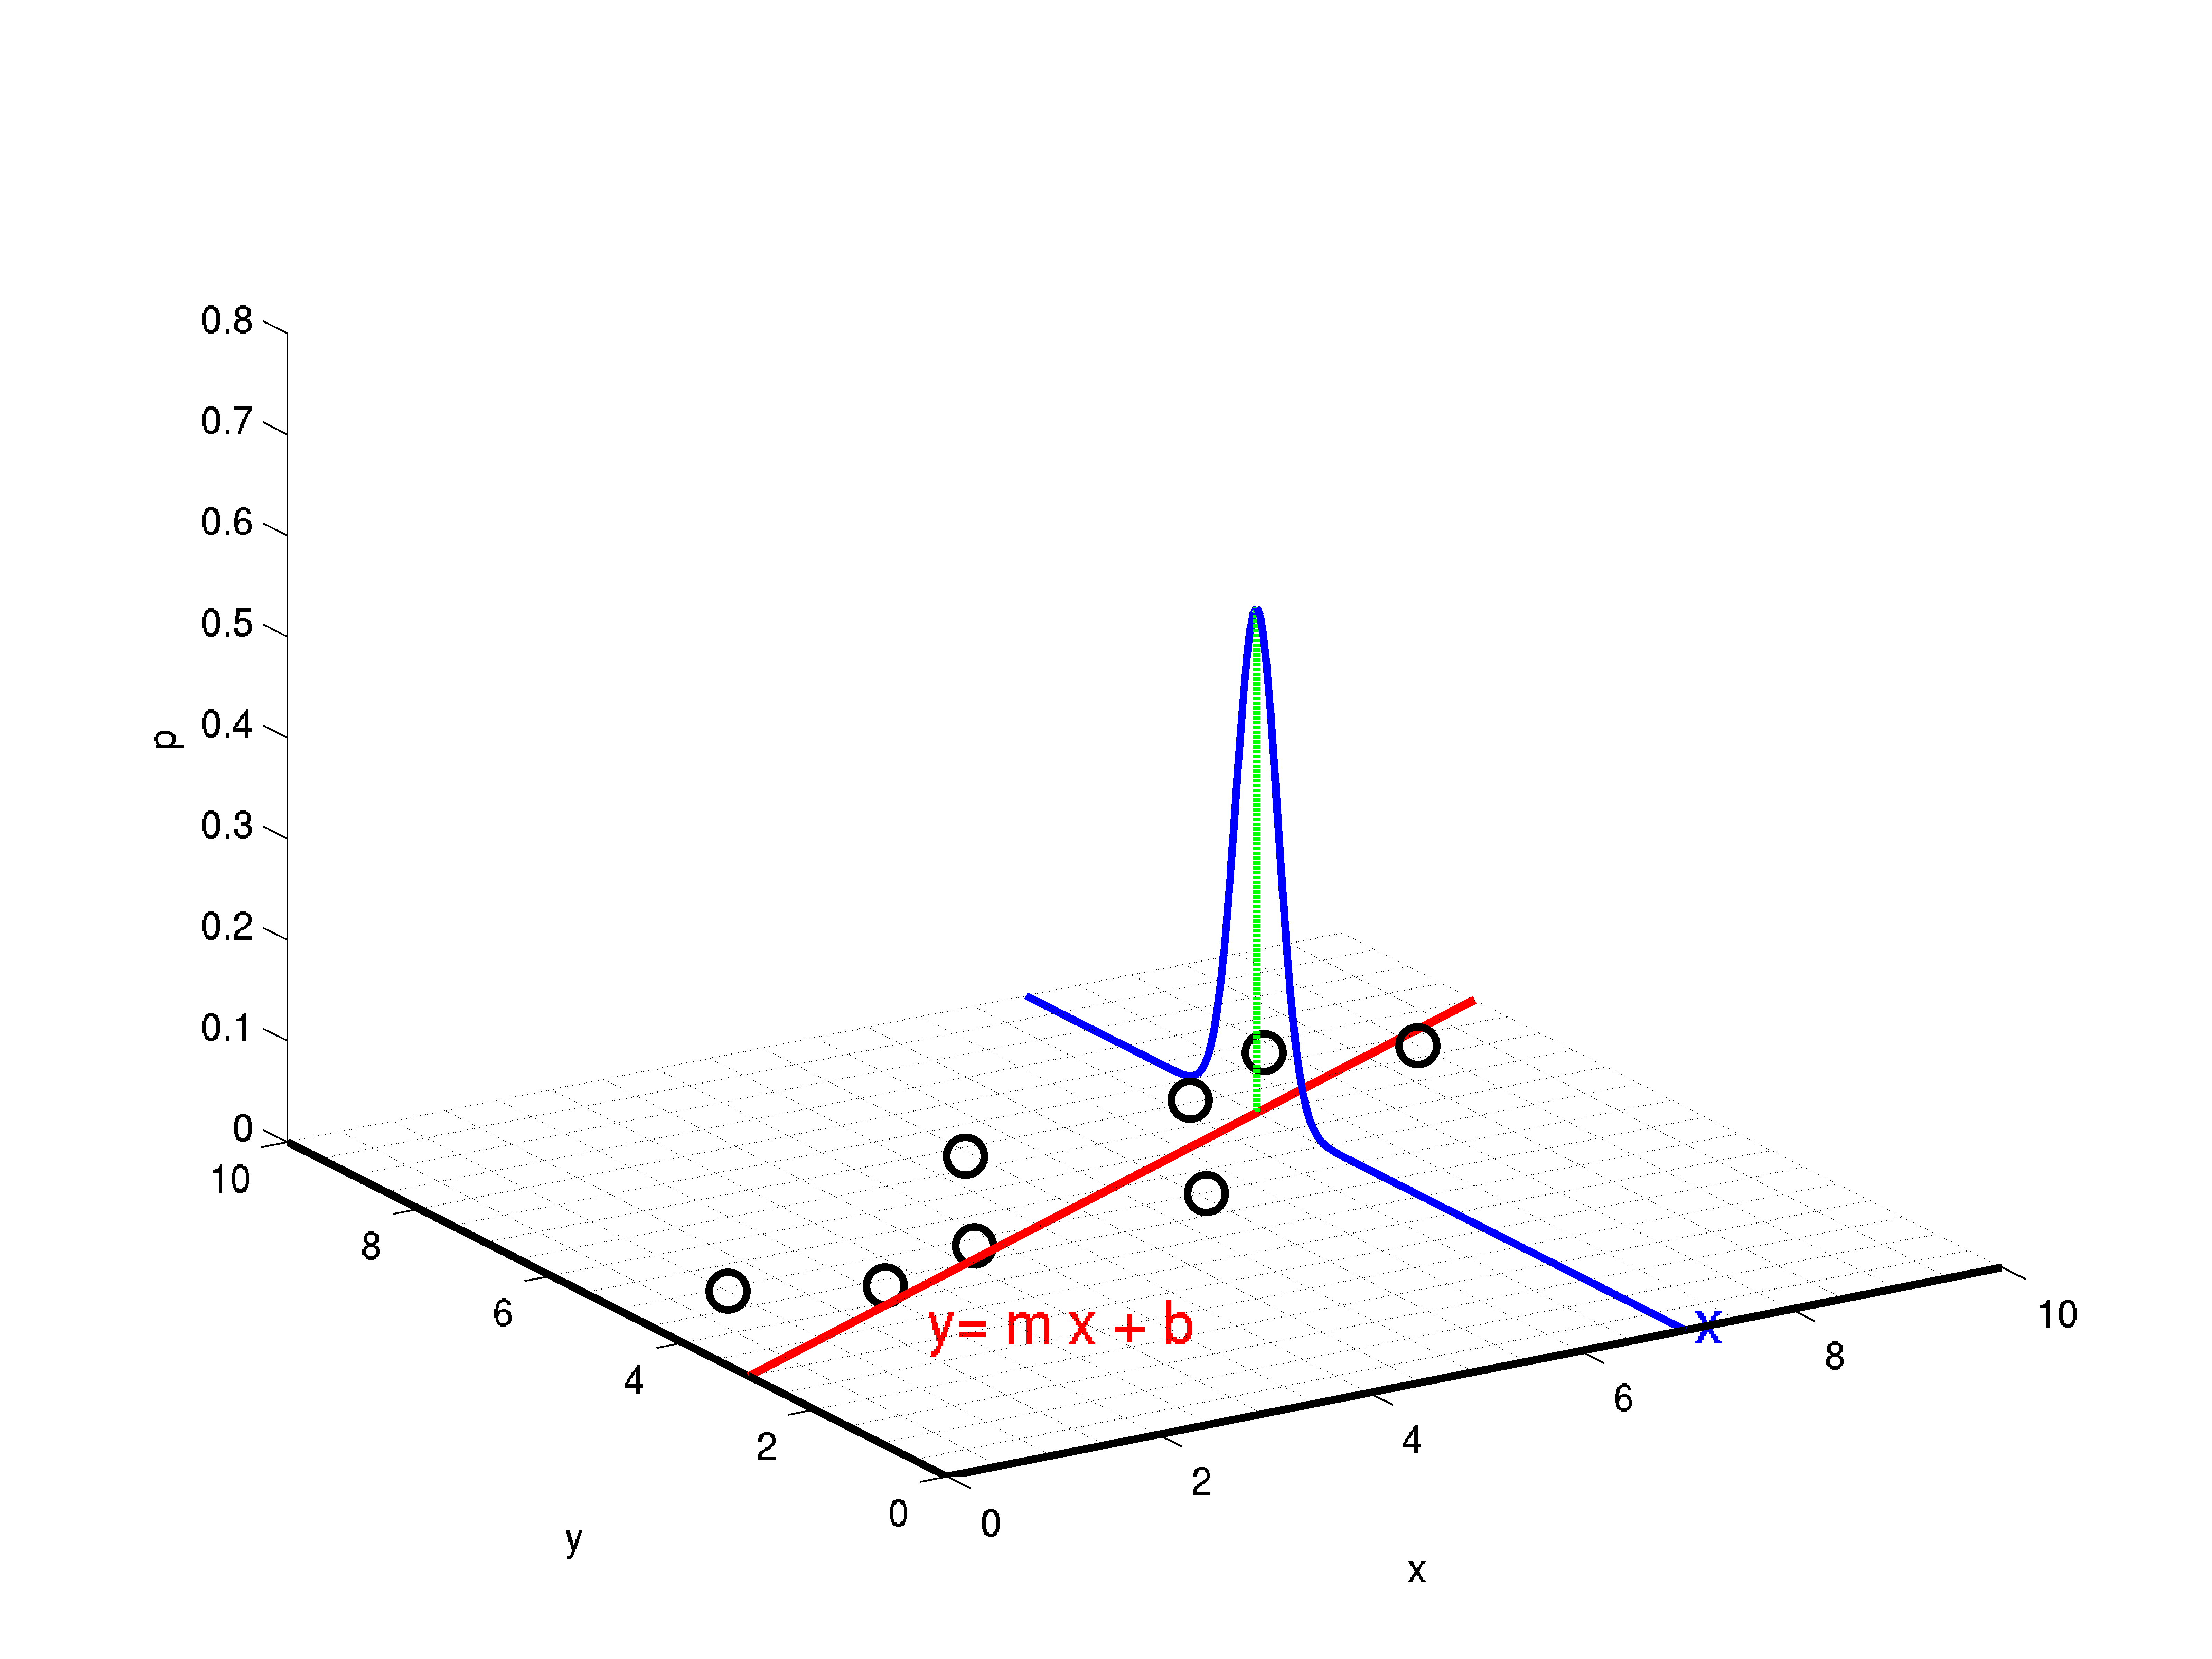
\includegraphics[width=5cm]{img/regressionInferenceThree}}
    }

  
\end{frame}

\begin{frame}
  \frametitle{The Predicted Value}

  The predicted value is 
  \begin{eqnarray*}
    \hat{y} & = & \hat{\beta}_1 x + \hat{\beta}_0.
  \end{eqnarray*}


  The predicted value  satisfies a $t$-distribution by
  \begin{eqnarray*}
    t & = & \frac{\hat{y}-y_{\mathrm{true}}}{\hat{\sigma}_y \sqrt{\frac{1}{n}+\frac{(x-\bar{x})^2}{S_{xx}}}},
  \end{eqnarray*}
  with $n-2$ degrees of freedom.

  \only<2->
  {

    \begin{columns}

      \column{.5\textwidth}
      Confidence Intervals:
      \begin{eqnarray*}
        t^* & = & \frac{\mathrm{error}}{\hat{\sigma}_y \sqrt{\frac{1}{n}+\frac{(x-\bar{x})^2}{S_{xx}}}},
      \end{eqnarray*}
      with $n-2$ degrees of freedom.

      \column{.5\textwidth}

      Hypothesis Testing:
      \begin{eqnarray*}
        t & = & \frac{\hat{y}-y_{\mathrm{true}}}{\hat{\sigma}_y \sqrt{\frac{1}{n}+\frac{(x-\bar{x})^2}{S_{xx}}}},
      \end{eqnarray*}
      with $n-2$ degrees of freedom.

    
    \end{columns}
  }


\end{frame}

\begin{frame}
  \frametitle{Side Note!}

  The predicted value is 
  \begin{eqnarray*}
    \hat{y} & = & \hat{\beta}_1 x + \hat{\beta}_0.
  \end{eqnarray*}


  The predicted value  satisfies a $t$-distribution by
  \begin{eqnarray*}
    \only<1>{t & = & \frac{\hat{y}-y_{\mathrm{true}}}{\hat{\sigma}_y\sqrt{\frac{1}{n}+\frac{(x-\bar{x})^2}{S_{xx}}}},}
    \only<2>{t & = & \frac{\lp \hat{\beta}_1 x + \hat{\beta}_0 \rp - \lp \beta_1 x + \beta_0\rp}{
        \hat{\sigma}_y\sqrt{\frac{1}{n}+\frac{(x-\bar{x})^2}{S_{xx}}}},}
  \end{eqnarray*}
  with $n-2$ degrees of freedom.
  
\end{frame}

\begin{frame}
  \frametitle{Inference on the Intercept Parameter}

  Let $x=0$, and we get 
  \begin{eqnarray*}
    t & = & \frac{\hat{\beta}_0 - \beta_0}{
        \hat{\sigma}_y\sqrt{\frac{1}{n}+\frac{(x-\bar{x})^2}{S_{xx}}}},
  \end{eqnarray*}
  with $n-2$ degrees of freedom.
  
\end{frame}

\section{Examples}

\begin{frame}{Example}

    \begin{columns}
      \column{.15\textwidth}

      \begin{tabular}{l|l}
        $X$ & $Y$ \\ \hline
        1 & 5.0 \\
        2 & 7.1 \\
        3 & 9.0 \\
        4 & 10.9 \\
      \end{tabular}

      \column{.25\textwidth}

      \begin{eqnarray*}
        \hat{\beta_1} & = & 1.96, \\
        \hat{\beta_0} & = & 3.1, \\
        \hat{\sigma}_y & = & \sqrt{0.006} \\
        s_{xx} & = & 5, \\
        s_{yy} & = & 19.22, \\
        s_{xy} & = & 9.8. 
      \end{eqnarray*}


      \column{.6\textwidth}

      Determine the 95\% confidence interval for the value of $y$ at $x=2.4$.

    \end{columns}

    \only<2->{%
      The 95\% confidence interval is from 7.64 to 7.97 assuming a
      $t$-distribution with 2 degrees of freedom.  
    }


\end{frame}


\begin{frame}{Example}

    \begin{columns}
      \column{.15\textwidth}

      \begin{tabular}{l|l}
        $X$ & $Y$ \\ \hline
        1 & 5.0 \\
        2 & 7.1 \\
        3 & 9.0 \\
        4 & 10.9 \\
      \end{tabular}

      \column{.25\textwidth}

      \begin{eqnarray*}
        \hat{\beta_1} & = & 1.96, \\
        \hat{\beta_0} & = & 3.1, \\
        \hat{\sigma}_y & = & \sqrt{0.006} \\
        s_{xx} & = & 5, \\
        s_{yy} & = & 19.22, \\
        s_{xy} & = & 9.8. 
      \end{eqnarray*}


      \column{.6\textwidth}

      Determine the 95\% confidence interval for the value of $y$ at $x=5.0$.

    \end{columns}

    \only<2->{%
      The 95\% confidence interval is from 12.49 to 13.31 assuming a $t$-distribution with 2
      degrees of freedom.  }


\end{frame}

\subsection{Connections with ANOVA}

\begin{frame}
  \frametitle{Bivariate Data and ANOVA}

    \begin{columns}
      \column{.15\textwidth}

      \begin{tabular}{r|r} % 
        $X$ & $Y$ \\ \hline
        $x_1$ & $y_1$ \\
        $x_2$ & $y_2$ \\
        $\vdots$ & $\vdots$ \\
        $x_n$ & $y_n$ 
      \end{tabular}

      \column{.85\textwidth}
      \uncover<2->{%
        Calculate the following:
        \begin{eqnarray*}
          S_{xx} & = & \lp x_1 - \bar{x}\rp^2 + \cdots + \lp x_n - \bar{x} \rp^2, \\
          S_{yy} & = & \lp y_1 - \bar{y}\rp^2 + \cdots + \lp y_n - \bar{y} \rp^2, \\
          S_{xy} & = & \lp x_1 - \bar{x}\rp\lp y_1 - \bar{y}\rp + \cdots + \lp x_n - \bar{x} \rp\lp y_n - \bar{y}\rp, \\
          \hat{r} & = & \frac{S_{xy}}{\sqrt{S_{xx} S_{yy}}}.
        \end{eqnarray*}
      }
      \end{columns}


  \uncover<3->{%
    
    Note:\\
    \begin{eqnarray*}
      \mathrm{SST}  & = & (y_1-\bar{y})^2 + (y_2-\bar{y})^2 + \cdots + (y_n-\bar{y})^2, \\
      \mathrm{SSTr} & = & (\hat{y}_1-\bar{y})^2 + (\hat{y}_2-\bar{y})^2 + \cdots + (\hat{y}_n-\bar{y})^2, \\
      \mathrm{SSE}  & = & (y_1 - \hat{y}_1)^2 + (y_2 - \hat{y}_2)^2 + \cdots + (y_n-\hat{y}_n)^2, \\
      \Rightarrow \mathrm{SST} & = & \mathrm{SSTr} + \mathrm{SSE}.
    \end{eqnarray*}
  }

  \vfill
  
\end{frame}


\begin{frame}
  \frametitle{Coefficient of Determination}

  \begin{definition}[Coefficient of Determination]
    The coefficient of determination is defined to be
    \begin{eqnarray*}
      R^2 & = & \frac{\mathrm{SSTr}}{\mathrm{SST}}, \\
          & = & 1 - \frac{\mathrm{SSE}}{\mathrm{SST}}.
    \end{eqnarray*}
  \end{definition}

  \uncover<2->{%
    The coefficient of determination represents the percent of change
    in the $y$ data that can be attributed to the change in the $x$
    data.  
  }
  

\end{frame}


%%% Local Variables: 
%%% mode: latex
%%% TeX-master: "IntroStats"
%%% End: 

% LocalWords:  pausesection hideothersubsections sectionstyle
